\documentclass[10pt,twocolumn]{article}
\usepackage[margin=0.75in,columnsep=0.28in]{geometry}
\usepackage{mathptmx}
\usepackage[T1]{fontenc}
\usepackage[utf8]{inputenc}
\usepackage{graphicx}
\usepackage{booktabs}
\usepackage{microtype}
\usepackage[hidelinks]{hyperref}
\usepackage{caption}
\captionsetup{font=small,labelfont=bf}
\graphicspath{{figs/}}
\setlength{\parskip}{2pt}

\title{\bfseries The Quiet Rewrite: Measuring the Organic Adoption and Consequences of LLM-Assisted Writing in Online Petitions, 2011--2024}
\author{Shahar Navian\\[2pt]\small Ben-Gurion University of the Negev \,\textperiodcentered\, \texttt{navians@post.bgu.ac.il}}
\date{}

\begin{document}
\maketitle
\vspace{-2em}

\begin{abstract}
\noindent Online petitions are among the most consequential texts ordinary citizens write, yet nothing is known about how many of them are now drafted with large language models (LLMs). We assemble 1.33 million petitions (2011--2024) spanning five government platforms (United Kingdom, Canada, Scotland, Russia; Korea as a pre-2022 anchor) and 773{,}000 cleaned English petitions (from a 964{,}636-petition public release) from the world's largest commercial platform, Change.org, and estimate LLM-style prevalence with a dictionary-free, split-half excess-vocabulary lower bound alongside pre-registered causal designs. By 2024, at least 18\% of UK parliamentary petitions and 8--12\% of Change.org petitions bear detectable LLM vocabulary---floors, not ceilings. Adoption is organic: Australia, which lacked Change.org's built-in AI tool until December 2023, shows a 4.9\% floor beforehand that doubles, with separated confidence intervals, the quarter the tool arrives. Repeat writers identified by user ID shifted their own style by $+0.62$\,SD, ruling out compositional explanations, and a language model trained solely on pre-ChatGPT petitions finds post-2022 text increasingly predictable---the low-entropy fingerprint of machine generation---while passing its pre-period falsification exactly. The consequences are ironic: LLM-styled petitions attract 7--13\% fewer signatures, are 15--19\% less likely to reach response thresholds, and lost the moderation advantage stylish writing enjoyed before 2022. All 27 identified threats to validity are tracked in a computed audit; all confirmatory hypotheses and analysis decisions were specified in advance in the released code.
\end{abstract}

\noindent\textit{Keywords:} large language models; e-petitions; AI-generated text; civic participation; computational social science

\section{Introduction}
Within two years of ChatGPT's release, LLM-flavoured prose has been documented in peer reviews, scientific abstracts, consumer complaints, and press releases \cite{liang2024monitoring,liang2025quantifying,kobak2025delving,patterns2025complaints}. Citizen petitions---texts whose explicit purpose is to persuade governments and fellow citizens---remained unmeasured. The closest study, Corpus et al.\ \cite{corpus2026introducing}, evaluated Change.org's own built-in writing assistant with a difference-in-differences design and found that outputs changed while outcomes did not; but a platform experiment cannot say how much of the petition ecosystem is being rewritten \emph{organically}, by people bringing their own chatbots, nor whether government portals---which offer no writing tools---are affected at all. Related evidence now spans political communication \cite{russo2025llm}, parliamentary text \cite{suvanto2026parl}, and the signature dynamics of petitioning itself \cite{yasseri2017rapid}; methodologically, we follow the fixed-false-positive-rate evaluation ethos of \cite{dugan2024raid} to its logical end by avoiding per-document detection altogether.

This paper provides those measurements. Our contributions are: (i)~the first cross-platform prevalence estimates of LLM-assisted writing in petitions, using a distributional lower bound that requires no per-document detector and therefore inherits none of the well-documented false-positive problems that burden detection of non-native writing \cite{liang2023gpt}; (ii)~a within-writer identification: because the Change.org release links petitions to stable user IDs, we show the \emph{same individuals} changed their writing, separating behavioural change from population turnover; (iii)~a generative falsification test in which a language model trained only on pre-2022 petitions quantifies, quarter by quarter, how far post-2022 text departs from the human baseline; and (iv)~outcome analyses---signatures, response thresholds, and moderation---showing that machine-styled petitions underperform.

\section{Data}
\textbf{Government platforms.} We collect the complete archives of five UK Parliament petition sites (2011--2024; the 2019 Parliament archive uniquely spans the ChatGPT cutover with 37{,}485 petitions before and 7{,}369 after), the Scottish Parliament, Russia's ROI, a partial Canadian House of Commons sample, and 398{,}935 Korean Blue House petitions that serve as a large pre-2022 anchor. Rejection codes, published by the UK and harmonized across parliaments, provide a moderation outcome unavailable on commercial platforms.

\textbf{Change.org.} We use the public release accompanying \cite{corpus2026introducing}: 964{,}636 English petitions (January 2022 -- December 2024) with original-casing text, titles, creation timestamps, author user IDs, per-petition country codes, and signature counts snapshotted on 9 January 2025. A computed reliability audit reconciles the release's three ID files to the paper's reported $N$ to within one record (1{,}517{,}432 unique of 1{,}517{,}433; one boundary duplicate; zero conflicting user IDs; zero timestamp disagreements in a 50{,}000-ID sample), and identifies the 552{,}796-record remainder as the non-English share. Because Change.org's in-platform AI tool reached the US, UK and Canada from April--October 2023 but Australia only on 15 December 2023, we split the platform into a \emph{treated} panel, an Australian \emph{organic} panel, and the remaining countries (the Philippines, notably, is the release's second-largest source with 104{,}000 petitions). Table~\ref{tab:corpus} summarizes.

\begin{table*}[t]\centering\small
\caption{Corpus composition (post-cleaning; cutover 30 Nov 2022). Scotland and Russia omitted for space ($n<500$).}
\label{tab:corpus}
\begin{tabular}{llrrrl}
\toprule
Source & Type & Lang & Pre & Post & Role\\
\midrule
UK 2010/2015/2017 archives & government & en & 99{,}467 & 0 & pre-era anchors\\
UK 2019 Parliament & government & en & 37{,}485 & 7{,}369 & primary contrast\\
UK current Parliament & government & en & 0 & 14{,}379 & post-only\\
Canada (partial) & government & en & 1{,}533 & 472 & underpowered\\
Korea Blue House & government & ko & 398{,}935 & 0 & anchor\\
Change.org US/GB/CA & commercial & en & 172{,}760 & 357{,}105 & tool-treated\\
Change.org Australia & commercial & en & 10{,}488 & 22{,}112 & organic panel\\
Change.org other countries & commercial & en & 63{,}142 & 147{,}446 & replication\\
\bottomrule
\end{tabular}
\end{table*}

\section{Methods}
\textbf{Style measurement.} Marker counts are computed on NFKC/quote/dash-normalized text and $z$-anchored within each platform's own pre-2022 distribution, so raw scores are never compared across platforms or languages. Lexical diversity uses MTLD \cite{mccarthy2010mtld} rather than the length-confounded type--token ratio. Every document carries a weight combining MinHash near-duplicate collapse (which also revealed 622 template campaigns spanning multiple platforms), NMF topic reweighting, and length-decile balancing; weighting reduces the pre/post length imbalance from a standardized difference of 0.58 to $-0.01$.

\textbf{Prevalence lower bound.} Following the excess-vocabulary logic of \cite{kobak2025delving}, we compare each word's post-2022 document frequency to a counterfactual anchored on the platform's own pre-period, and define $\pi_{\mathrm{lb}}(q)$ as the share of quarter-$q$ documents containing at least one excess word, minus the counterfactual share. Three safeguards make this an honest floor: words are selected on a hash-defined half of the post-era and prevalence is estimated on the other half; placebo words, NMF topic words and a news stoplist are banned; and any LLM output using only vocabulary humans already used is invisible to the method by construction.

\textbf{Causal designs.} The UK 2019 archive supports an event study with a 400-permutation placebo-date null and a fixed-effects interrupted time series estimated identically on a placebo outcome (common words with no documented LLM excess). On Change.org, stable user IDs enable a within-writer fixed-effects estimate for the 7{,}250 authors active in both eras. As a model-free falsification, we fine-tune a small causal LM (distilgpt2) exclusively on pre-cutover petitions and track per-token surprise on later quarters; pre-cutover evaluation quarters must sit at ratio 1.0 for the design to be valid. Signature models use quasi-Poisson with creation-to-snapshot exposure and, as growth-immune variants, within platform$\times$quarter percentiles and platform$\times$quarter fixed effects---so rising internet adoption cannot manufacture an effect. Confirmatory hypotheses (H1--H4) and every analysis decision were frozen in the pipeline's code --- which generates the analysis-plan document verbatim --- before any confirmatory result existed; a 27-item audit computes the status of every identified threat to validity from the pipeline's own output files.

\section{Results}
\subsection{Adoption is large, organic, and cross-platform}
Figure~\ref{fig:es} shows the UK 2019 event study: eleven pre-cutover quarters are flat (maximum coefficient 0.078\,SD, below the pre-specified 0.10 bar), followed by a ramp reaching $+0.21$\,SD three quarters and $+0.33$\,SD five quarters after ChatGPT's release. None of 400 placebo cut-dates produces an effect as large as the real one (0.132 vs.\ a null SD of 0.021). The replication forest (Figure~\ref{fig:forest}) repeats the within-platform contrast everywhere data permit: standardized shifts of 0.29--0.46 on the three Change.org panels and 0.11 on the UK, with the placebo score at zero in every panel.

\begin{figure*}[t]\centering
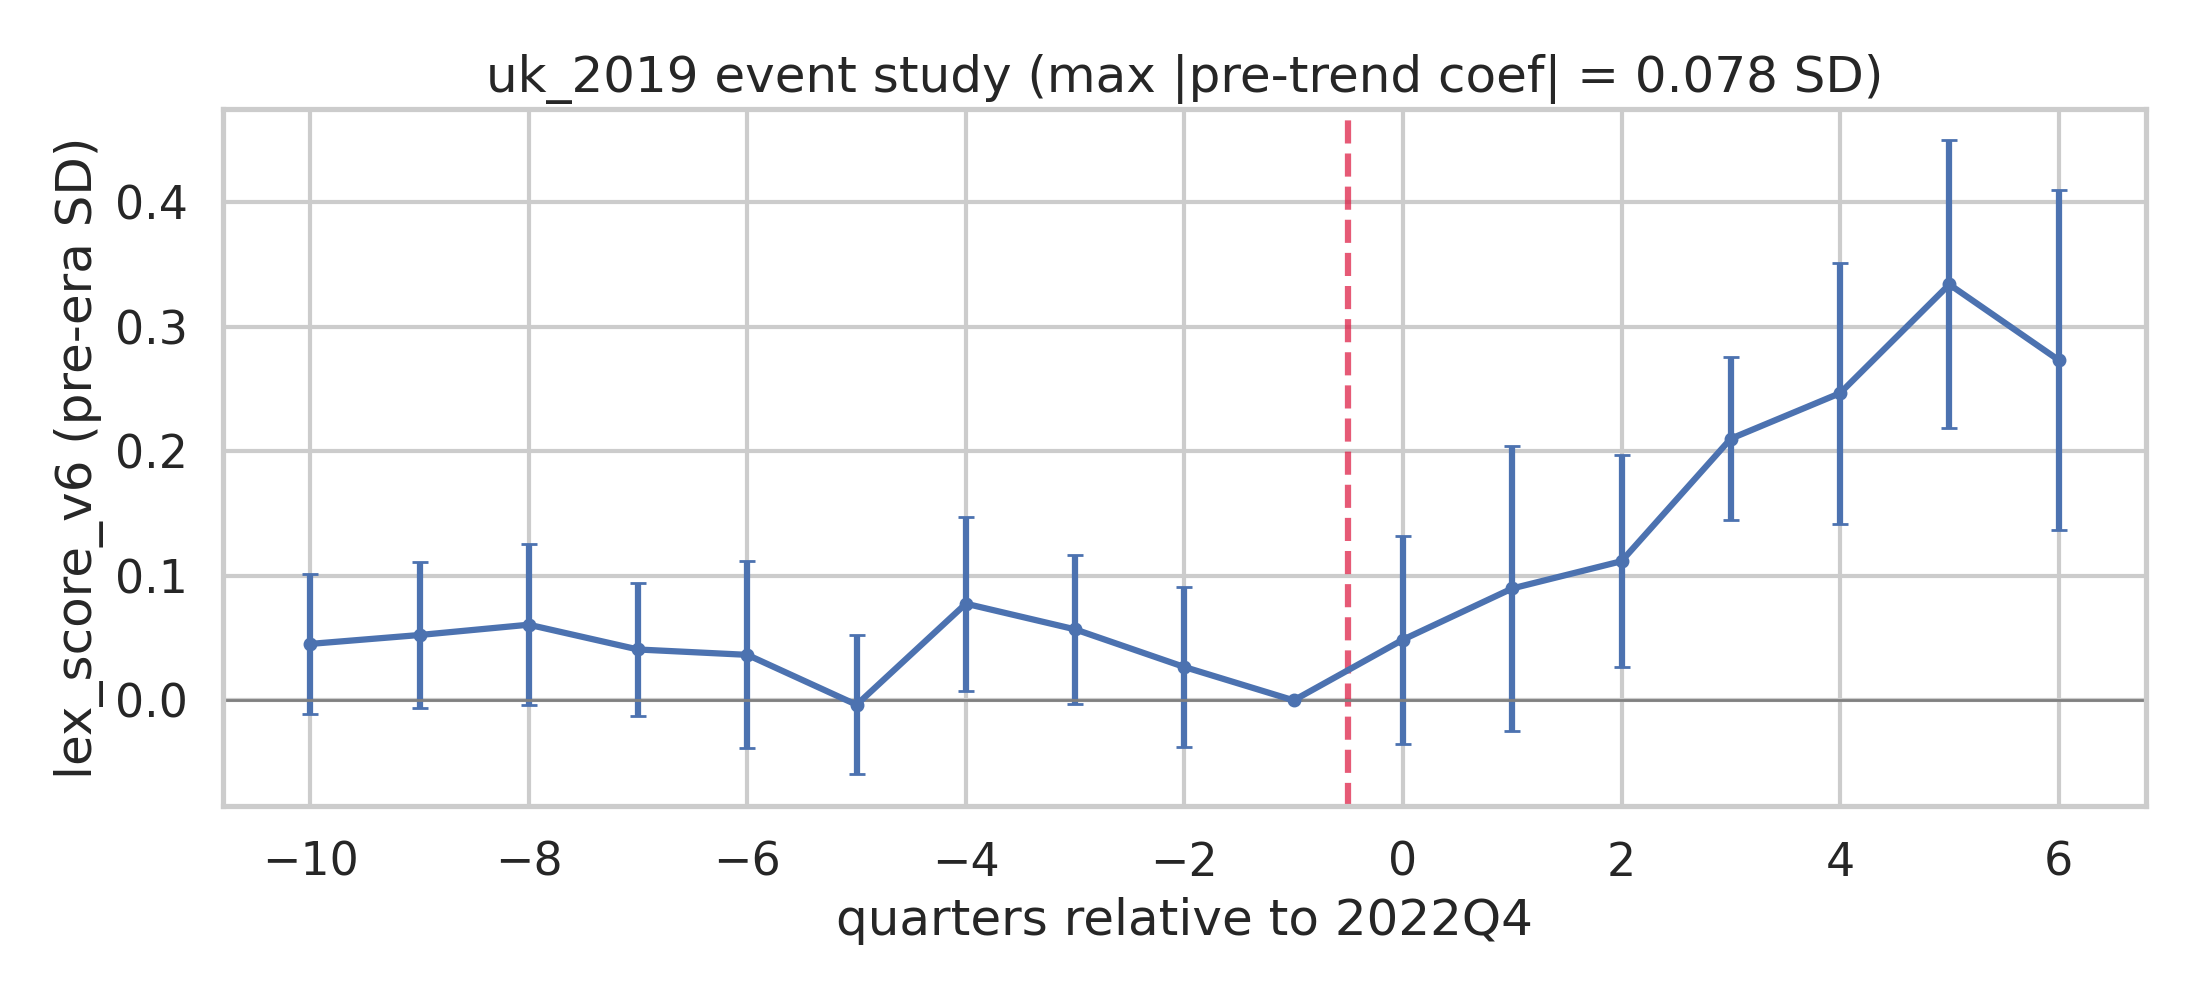
\includegraphics[width=.78\textwidth]{FIG_V6_eventstudy.png}
\caption{UK 2019 Parliament event study; 95\% CIs, week-clustered. The dashed line marks 2022Q4.}
\label{fig:es}
\end{figure*}

\begin{figure}[t]\centering
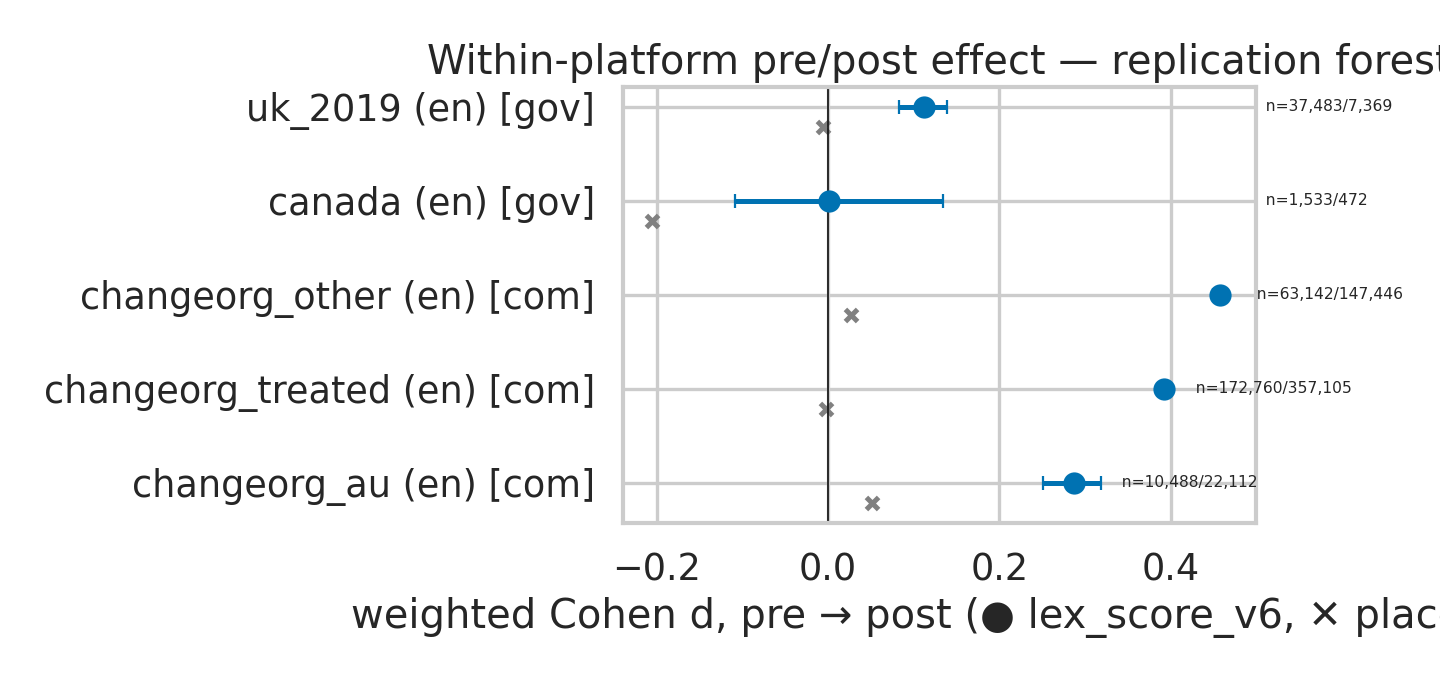
\includegraphics[width=\columnwidth]{FIG_V6_forest.png}
\caption{Within-platform pre$\rightarrow$post effects ($\bullet$ lexical score; $\times$ placebo). Canada is underpowered (partial collection).}
\label{fig:forest}
\end{figure}

The prevalence floors (Figure~\ref{fig:prev}) are the headline. UK parliamentary petitions reach $\pi_{\mathrm{lb}} = 17.9\%$ $[14.5, 21.6]$ by 2024Q1; a conservative variant that replaces the trend counterfactual with the pre-period mean---immune to COVID-vocabulary mean-reversion---selects 35 clean register words (\emph{believe, require, urge, significant, accountable}\,\ldots) and yields a converging single-word floor of 18.6\% (``believe'' alone rises from 8.2\% to 26.8\% of documents). On Change.org the treated panel climbs smoothly to 7.9\% $[7.6, 8.1]$ by end-2024. Australia is the study's natural experiment: with no in-platform tool, its organic floor is 4.9\% $[3.0, 6.6]$ in 2023Q4---consistent, as a lower bound, with the ${\approx}18\%$ classifier estimate of \cite{corpus2026introducing}---and jumps to 11.6\% $[10.4, 13.1]$, confidence intervals fully separated, in the exact quarter the tool arrives. The word lists themselves converge with an independent dictionary-free scan of the whole corpus, whose top excess words (\emph{perpetuates, embrace, deeply, innovative, addressing}) reproduce the documented LLM register \cite{kobak2025delving}.

\begin{figure*}[t]\centering
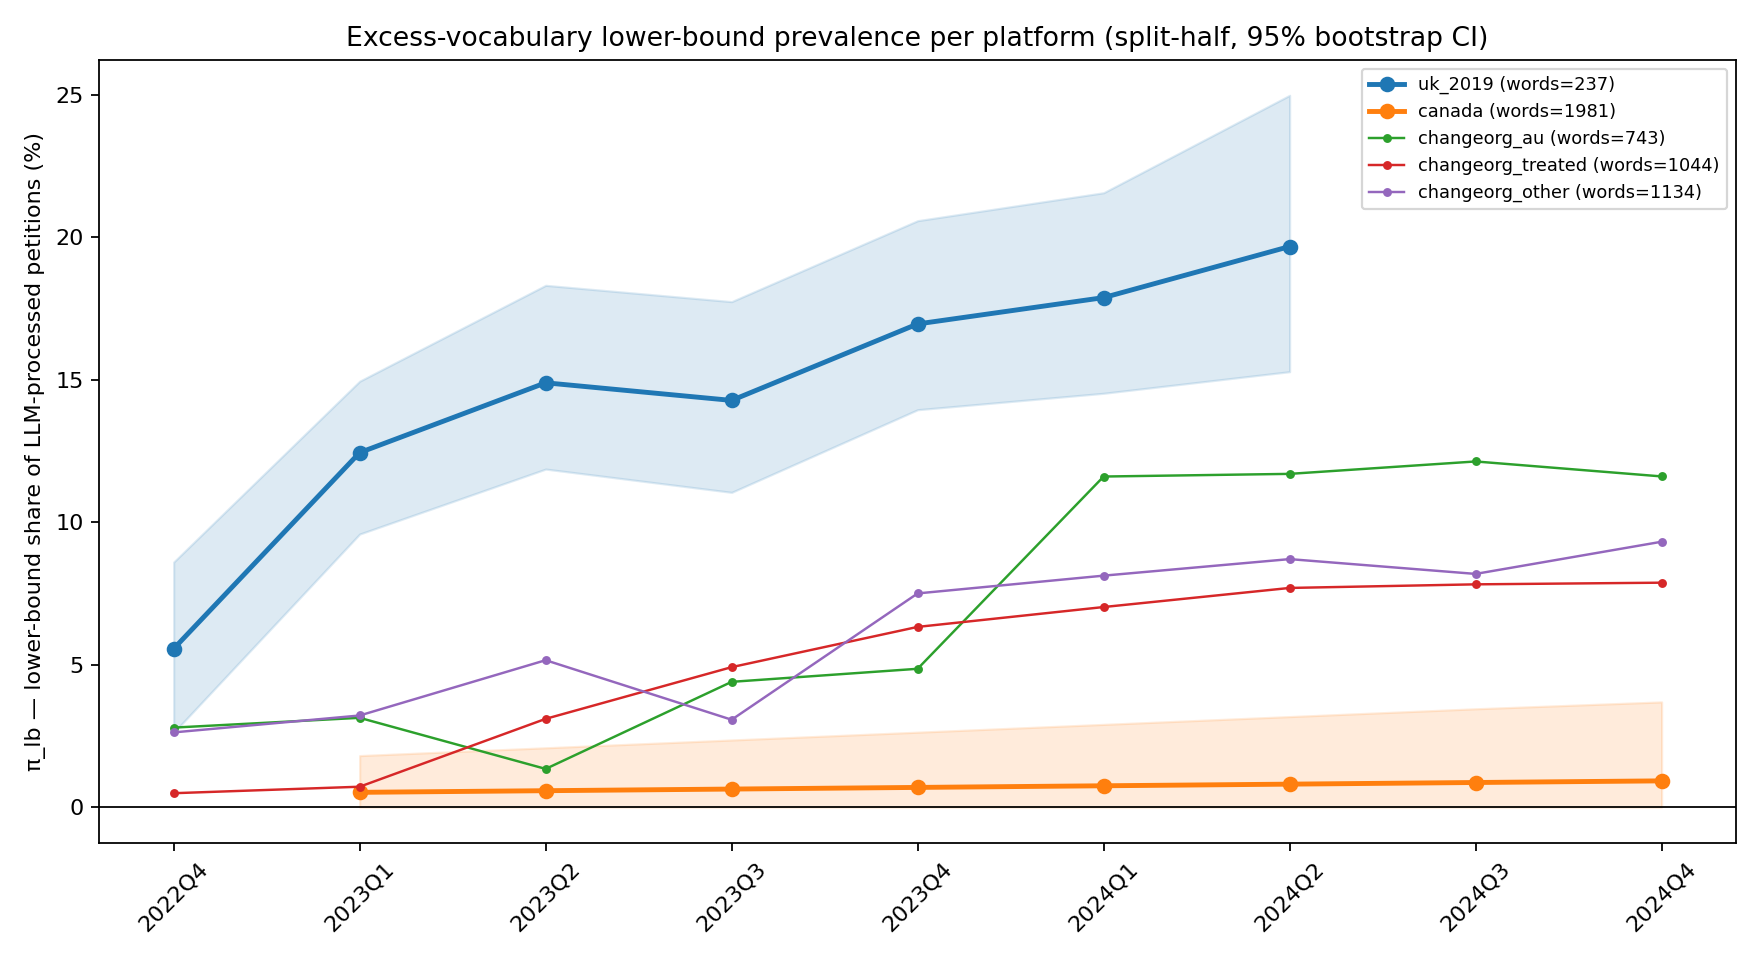
\includegraphics[width=.8\textwidth]{FIG_V6_prevalence.png}
\caption{Excess-vocabulary lower-bound prevalence $\pi_{\mathrm{lb}}$ per platform (split-half selection/estimation; 95\% bootstrap CIs).}
\label{fig:prev}
\end{figure*}

\subsection{The same people changed}
Because every Change.org petition is linked to its author, composition and behaviour separate cleanly. Among 7{,}250 writers active in both eras (23{,}043 petitions), the within-writer fixed-effects shift is $+0.62$\,SD (clustered $p<10^{-15}$); it is $+0.37$\,SD in the organic Australian subset. One quarter (25.4\%) of repeat writers jumped by more than a full standard deviation (Figure~\ref{fig:ww}), while post-era newcomers write another $+0.59$\,SD above returning authors---both channels are real, but neither turnover nor topic drift can explain the within-person change. Adoption has not made petitioning faster: within-era gaps between a writer's consecutive petitions are no shorter after 2022, and the share of output from first-time authors declined (96\% $\rightarrow$ 85\%).

\begin{figure}[t]\centering
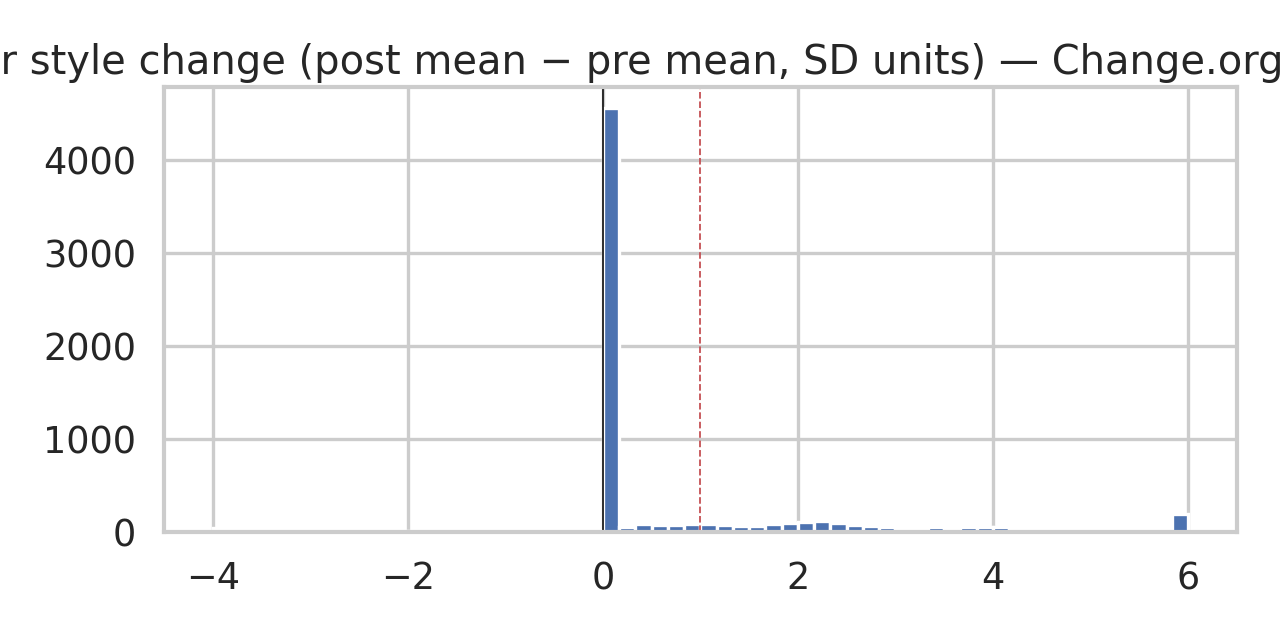
\includegraphics[width=.92\columnwidth]{FIG_V6_within_writer.png}
\caption{Per-writer style change (post mean $-$ pre mean) among Change.org authors active in both eras.}
\label{fig:ww}
\end{figure}

\subsection{What changed in the language}
A pre-2022 language model finds later petitions \emph{easier}, not harder, to predict (Figure~\ref{fig:lm}): surprise ratios sit at 0.99--1.01 across every pre-cutover falsification quarter, then fall to 0.945 $[0.928, 0.965]$ on the UK by 2024Q1 and to 0.864 $[0.849, 0.879]$ on Change.org by 2023Q4---the low-entropy signature of model-generated text, obtained without any detector. Embedding analyses show semantic homogenisation on Change.org (mean pairwise similarity $0.102 \rightarrow 0.125$ in the treated panel) alongside stylometric era-separability (character-$n$-gram probe AUC 0.74--0.81; within-topic semantic AUC 0.62--0.67, so news drift does not explain it). Yet the population is polarizing rather than uniformly drifting: the variance of the style score explodes post-2022 (UK $0.97 \rightarrow 1.78$; treated $0.99 \rightarrow 4.24$), a mixture of adopters and abstainers. Titles tell the interface story: on Change.org they lengthen, double their ``X: Y'' colon rate, and drift lexically from the body at constant semantic alignment---the signature of paraphrased, machine-drafted titles---while on the UK portal, which suggests nothing, every title metric is unchanged (colon share $0.006 \rightarrow 0.006$).

\begin{figure*}[t]\centering
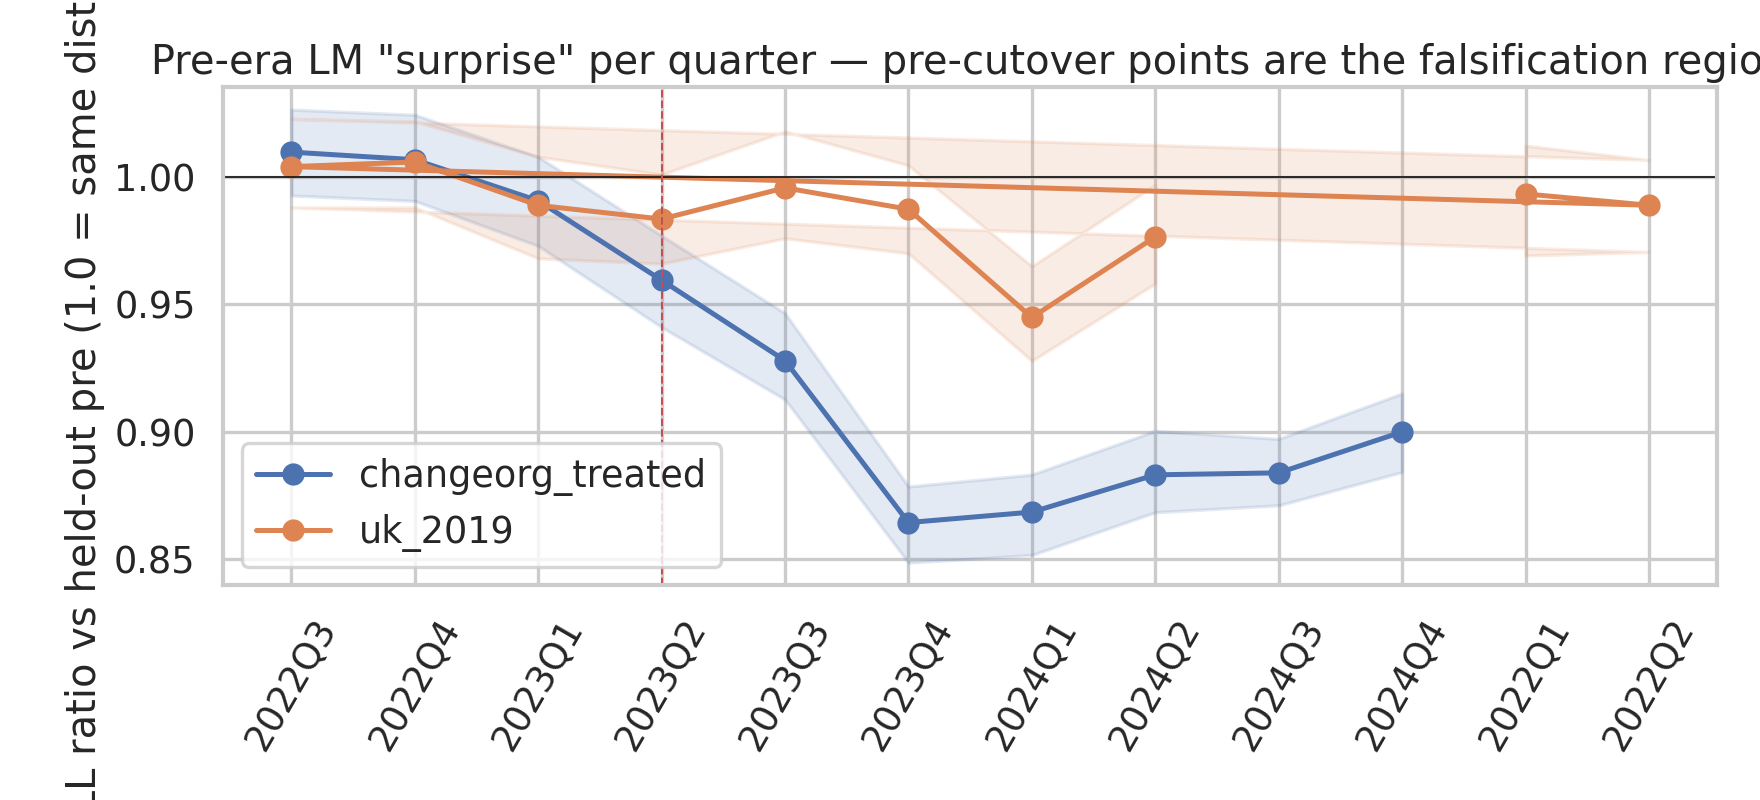
\includegraphics[width=.75\textwidth]{FIG_V6_lm_surprise.png}
\caption{Per-quarter surprise of a pre-2022-trained LM (NLL ratio vs.\ held-out pre-era; 1.0 = same distribution).}
\label{fig:lm}
\end{figure*}

\subsection{It does not help}
Before 2022, polished register was neutral-to-mildly advantageous: the same signature model that is null in the pre-era benchmark ($+2.0\%$, $p=.26$) turns negative after---$-7.0\%$ signatures per $+1$\,SD of LLM style in the growth-immune platform$\times$quarter specification, $-12.6\%$ on UK 2019 alone---and stylish post-era petitions are 15\% and 19\% less likely to reach the 10{,}000- and 100{,}000-signature thresholds (interaction ORs 0.85 and 0.81). Moderation flips the same way: a standard deviation of style predicted fewer rejections before 2022 (OR 0.96) and more after (interaction OR 1.06). Whether readers penalize recognizably synthetic prose or the tool flattens persuasive specificity, the widespread private bet that an LLM improves a petition's chances finds no support---extending the platform-experiment null of \cite{corpus2026introducing} to organic use and to government portals.

\section{Robustness and limitations}
One pre-specified criterion failed informatively: the interrupted-time-series step at the ChatGPT date is null everywhere because adoption is gradual; effects load on later dose dates, and under an amended rule anchoring on the largest dose---with the placebo counted only when it moves in the same direction---specificity passes in all four samples (the placebo in fact moves \emph{opposite} to the effect, the reverse of the composition artifact that motivated the design). Remaining limitations are declared rather than hidden: the Change.org pre-window is short (January--November 2022) and its release excludes petitions deleted before the January 2025 snapshot; post-2023Q4 commercial estimates mix organic and in-platform tool use (the Australian panel isolates organic use through 2023Q4 only); Canada's collection is partial and its null is uninformative; marker-based shifts are upper bounds on direct LLM use (professionalisation-risk vocabulary carries 60\% of the UK marker gap, which is precisely why the headline estimators are dictionary-free); $\pi_{\mathrm{lb}}$ is a floor by construction; MTLD retains a moderate length correlation ($\rho=.52$); Korean supplies an anchor but no post-era contrast; and author identifiers exist only on the commercial platform. Every one of the 27 audited threats, including these, carries a computed status in the released audit table.

\section{Conclusion}
Between late 2022 and the end of 2024, machine-assisted drafting became a routine, uninvited participant in petitioning: at least one in six UK parliamentary petitions and one in twelve Change.org petitions carry its vocabulary, the same citizens who once wrote unaided now write with it, and the language of collective demand is measurably converging on a register that a two-year-old model of human petitions finds ever less surprising---while persuading fewer people. For platforms and parliaments, the finding cuts both ways: there is no epidemic of successful synthetic manipulation to fear, and no participatory dividend to celebrate; there is instead a quiet homogenisation of civic voice whose long-run costs---to authenticity signals, to moderation, to the informational value of petition text---deserve measurement of exactly the kind this pipeline, released with its frozen analysis plan, audit, and code, is built to repeat.

\section*{Acknowledgments}
In accordance with the course policy on tool use: this project made extensive use of \emph{Claude} (Anthropic) as an AI assistant throughout --- for research design consultation, literature discovery, implementation and debugging of the analysis pipeline, verification of results, and drafting and editing of this paper. All analytical decisions, the interpretation of results, and the final text were reviewed by, and are the sole responsibility of, the author. Additional tools: Google Colab (A100), Python (pandas, statsmodels, scikit-learn, datasketch, sentence-transformers, transformers), and Google Drive.

\paragraph{Data and code availability.} The full pipeline (a documented Colab notebook), the frozen analysis plan, the 27-item bias audit, and all aggregate result tables and figures are submitted via a private GitHub repository shared with the course staff. Change.org data are available from the public release of \cite{corpus2026introducing} (osf.io/q3hj5) and are not redistributed; UK, Scottish, Canadian and Russian petition data are public records collected from the respective official portals; the repository documents how to obtain each source.

\begin{thebibliography}{12}\footnotesize
\bibitem{liang2024monitoring} W. Liang et al. Monitoring AI-modified content at scale: LLMs in AI conference peer reviews. \emph{ICML}, 2024. arXiv:2403.07183.
\bibitem{liang2025quantifying} W. Liang et al. Quantifying LLM usage in scientific papers. \emph{Nature Human Behaviour}, 2025. doi:10.1038/s41562-025-02273-8.
\bibitem{kobak2025delving} D. Kobak et al. Delving into LLM-assisted writing in biomedical publications through excess vocabulary. \emph{Science Advances}, 2025. doi:10.1126/sciadv.adt3813.
\bibitem{patterns2025complaints} W. Liang, Y. Zhang, M. Codreanu, J. Wang, H. Cao, J. Zou. The widespread adoption of large language model-assisted writing across society. 2025. arXiv:2502.09747.
\bibitem{corpus2026introducing} I. S. Corpus, S. Gilbert, A. Koenecke, M. Naaman. Introducing AI to an online petition platform changed outputs but not outcomes. 2026. arXiv:2511.13949.
\bibitem{dugan2024raid} L. Dugan et al. RAID: A shared benchmark for robust evaluation of machine-generated text detectors. \emph{ACL}, 2024. arXiv:2405.07940.
\bibitem{mccarthy2010mtld} P. M. McCarthy, S. Jarvis. MTLD, vocd-D, and HD-D: A validation study of sophisticated approaches to lexical diversity assessment. \emph{Behavior Research Methods} 42, 2010.
\bibitem{liang2023gpt} W. Liang et al. GPT detectors are biased against non-native English writers. \emph{Patterns} 4(7), 2023.
\bibitem{russo2025llm} G. Russo et al. Large language models in online political communication. \emph{CSCW}, 2025.
\bibitem{yasseri2017rapid} T. Yasseri, S. Hale, H. Margetts. Rapid rise and decay in petition signing. \emph{EPJ Data Science}, 2017.
\bibitem{suvanto2026parl} E. Suvanto et al. LLM style in parliamentary text: UK Hansard and Swedish Riksdag motions. 2026. arXiv:2606.14209.
\end{thebibliography}

\end{document}
